\documentclass{article}
\usepackage[a4paper, total={6in, 8in}]{geometry}
\usepackage{color}
\usepackage{xcolor}
\usepackage{listings}
\usepackage{parskip}
\usepackage{graphicx}
\usepackage{subcaption}
\usepackage{amsmath}
\usepackage{comment}
\usepackage[hidelinks]{hyperref}
\lstset{language=C++,
                keywordstyle=\color{blue},
                stringstyle=\color{red},
                commentstyle=\color{cyan},
                morecomment=[l][\color{magenta}]{\#},
                breaklines=true,
}
\newcommand{\auth}{\fontsize{11}{13}\selectfont}

\title{Assignment 3: Task Farming}
\author{\auth Group 16: Anton Marius Nielsen (kjq186), Asmus Tørsleff (qjv778)\\ \auth\& Ida Rye Hellebek (hcx206)}
\date{\auth February 2024}

\begin{document}
\maketitle

\section{Write functional task farming program}


%In the report, you should explain how you have parallelised the program.
%Remember to discuss when and what data you exchange between the MPI-processes and how that impacts the performance. It is up to you if you use blocking or non-blocking messages, or maybe both versions.

The basic principle for parallelisation in our program is that master loops through the tasks, sending each to the next available worker. In more detail this is achieved by:

\begin{enumerate}
    \item Sending out a task to each worker
    \item Waiting for a receive from any worker
    \item Storing result and sending new task to newly returned worker, until all tasks are sent
    \item Receiving last results, before sending a termination signal to returned workers
\end{enumerate}

In this simple case, the data we send from master to worker and vice versa is a reference to a single integer value. The referenced integer value received by master is used to identify the worker, though this could also be done by using the status.

The termination signal is tag = 1, whereas all other messages have tag = 0. 

We use blocking messages in all cases here, as there are little computation to do while waiting for a receive request. In a larger setup, with a higher risk of crashing or unavailable workers, it may be beneficial to adapt the setup to non-blocking send requests.

%% should we implement/benchmark with non-blocking?

\section{Task farming for HEP data}

We adapt our implementation of the master-worker program to the HEP data. The adaptions include:

\begin{itemize}
    \item changing size and type of the data exchanged between master and worker.
    \item using the status to identify workers
    \item keeping track of the task index to archive results at corresponding position
\end{itemize}

The latter is done by initializing an array of length nworkers for saving the last task index sent to each worker. This is used to archive accuracies in the right order, making sure that we can access the settings used to obtain the best accuracy.

\newpage

\section{Benchmarking on MODI}

\subsection*{A: Performance results}

% How you choose to distribute the MPI-processes between the MODI compute nodes and their CPU-cores is up to you. Remember to discuss briefly your decision in the report. 

With \lstinline{n_cuts = 4}, we benchmark the parallel implementation \lstinline{task_farm_HEP.cpp} on MODI, with an increasing number of processes. The number of processes shown in figure \ref{fig:perf} includes the master, meaning that the number of workers are one less. The data is also shown in appendix table \ref{fig:perf}.

All cores used are on the same compute node to make the comparison simple. Running on different nodes are expected to yield slightly lower speedup, because the message speed decrease when using the network between nodes.

\begin{figure}[h!]
    \begin{subfigure}{0.48\textwidth}
        \centering
        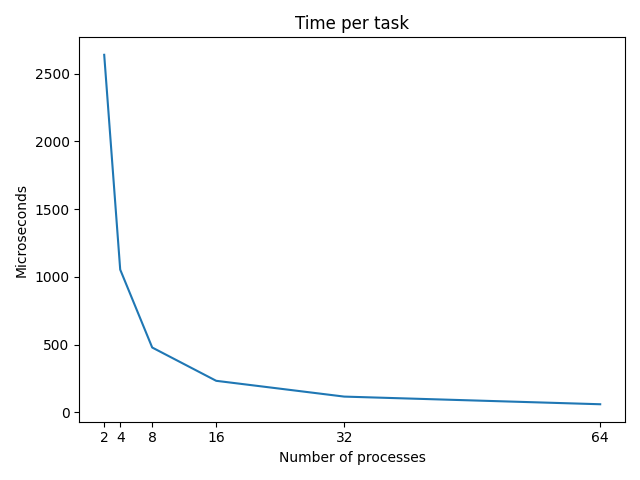
\includegraphics[width=\textwidth]{img/task_perf.png}
        \caption{Performance increase with number of processes}
        \label{fig:abs_perf}
    \end{subfigure}
    \begin{subfigure}{0.48\textwidth}
        \centering
        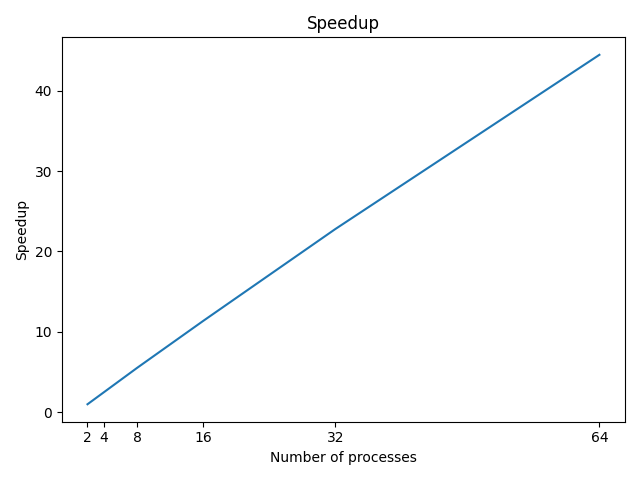
\includegraphics[width=\textwidth]{img/task_speedup.png}
        \caption{Speedup relative to having one worker}
        \label{fig:rel_perf}
    \end{subfigure}
    \caption{Absolute and relative performance}
    \label{fig:perf}
\end{figure}

From figure \ref{fig:rel_perf} the acieved speedup seems close to ideal speedup, indicating that only a small fraction of the code is serial. However, we know that some part of our code will be serial, and we would not expect ideal speedup for a larger range of processes.

\subsection*{B: Serial and parallel fractions}

% Estimate the serial and parallel fraction of the code in the context of Amdahl’s law. And plot a theoretical scaling curve for your results. Only consider the CPU cores dedicated to workers.

If we rearrange Amdahl's law, we can use it to calculate the parallel fraction ($P$) in the program. The baseline here is two processes (one worker, one master), and we use the number of workers as $N$ in the calculations.

\begin{equation*}
    Speedup(N) = \frac{1}{(1-P) + \frac{P}{N}} 
    \hspace{1em} \Leftrightarrow \hspace{1em}
    P = \frac{ {Speedup}^{-1} - 1}{{N}^{-1} - 1}
\end{equation*}

Using the speedup when running 64 processes (63 workers), we get a parallel fraction of 99.3\% and serial fraction of 0.7\%.

A theoretical scaling curve with this percentage is plotted in figure \ref{fig:theo}. From this, it is obvious that the near ideal speedup only applies with a limited number of processes.

\begin{figure}[h!]
    \centering
    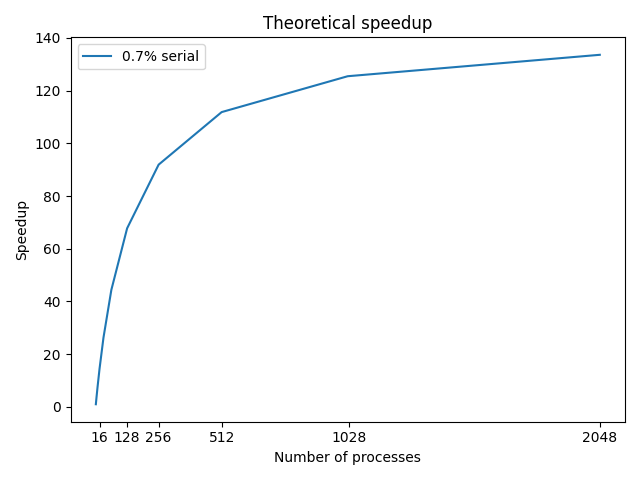
\includegraphics[width=0.6\textwidth]{img/theo_speedup.png}
    \caption{Theoretical scaling curve}
    \label{fig:theo}
\end{figure}


\subsection*{C: Discussion of strong scaling}

%Discuss your results in the context of strong scaling. What is your recommendation to the high-energy physicists in terms of limits for how many CPU cores they can employ, and if you benchmark more than one version of the code, does the relative scaling make sense?

Assuming that the parallel fraction is approximately 99.3\%, the gain in performance diminish when using more than a thousand processes. Thus, a maximum of thousand cores may be a reasonable advise for high energy physicists running this analysis.

However, one should be aware of that the hardware architechture for an increasing number of cores might lower the actual speedup. This can be a result of poor network connections and slower memory access. In this case, the most reasonable number of cores might be lower, depending on the exact hardware used.



\newpage

\section{Appendix}

\begin{table}[h!]
    \centering
    \caption{Performance as total elapsed time and time per task}
    \begin{tabular}{|c c c|} 
    \hline
    Number of processes & Seconds elapsed & µ seconds / task \\ \hline
    2 & 172.9 & 2638  \\ \hline
    4 & 69.02 & 1053  \\ \hline
    8 & 31.33 & 478  \\ \hline
    16 & 15.22 & 232.3 \\ \hline
    32 & 7.59 & 115.8 \\ \hline 
    64 & 3.89 & 59.3 \\ \hline
    \end{tabular}
    \label{tab:raw_perf}
\end{table}


%% don't know how to explain these data, so i left it all out, just using 64 processes

\begin{comment}
The calculated parallel fraction deviates slightly across number of workers (see \ref{tab:p_frac}), possibly due to hardware architechture and initial latency. We use the calculated parallel fraction when running 64 processes, because???

\begin{table}[h!]
    \centering
    \caption{Parallel fraction using Amdahl's law}
    \begin{tabular}{|l|l|l|l|l|l|}     \hline 
    Workers       & 3     & 7     & 15    & 31    & 63   \\ \hline
    Speedup       & 2.51  & 5.52  & 11.36 & 22.79 & 44.47 \\ \hline
    Parallel Frac & 0.901 & 0.955 & 0.977 & 0.988 & 0.993\\ \hline
    \end{tabular}
    \label{tab:p_frac}
\end{table}
\end{comment}

\newpage

\section{Implementation for task 1}

\lstinputlisting[language=c++]{task_farm.cpp}

\newpage

\section{Implementation for task 2}

\lstinputlisting[language=c++]{task_farm_HEP.cpp}

\end{document}
